\section{Introduction}

The theory of arithmetic
is among the most prolific theories used in SMT solvers. It is used across a wide set of
applications, and they have a wide range of demands.
Supporting efficient theory solvers for arithmetic requires balancing feature support,
ranging from linear, difference logic, to linear real, linear integer, non-linear polynomial arithmetic
and in cases transcendental functions such as exponentiation.
The aim of this paper is to provide a high-level, yet self-contained, overview of internal ingredients of the arithmetic solver.
It seeks to explain tool users what to expect of solving methodologies when using Z3 for arithmetic.
We assume familiarity of basics of SMT solving using CDCL(T), e.g.,~\cite{z3internals}.
While make an effort to cover all features for completeness,
we devote attention to highlight a selection that to our knowledge are unique for arithmetic solvers.
These highlights include
(1) how the solver patches linear real programming solutions to find solutions to integer variables,
(2) heuristics that are new in how the solver finds Gomory cuts, and
(3) the solver's integration of Gr{\"o}bner basis computation for solving non-linear constraints.
User pain points around SMT have to our experience centered dominantly
around quantifiers and non-linear arithmetic. A complete (for non-linear reals) solver that integrates
with other theories and quantifier reasoning becomes relevant. The new arithmetic solver that we describe here
was first integrated in version 4.8.8 of z3, turned on as default in the next release,
and subjected to later significant revisions.
To evaluate the contribution of each feature we use benchmarks drawn
from SMTLIB benchmark sets~\cite{SMTLIB2} and benchmarks supplied by a user, 
Certora~\cite{bench-submission}.

In overview, the arithmetic solver uses a waterfall model for solving arithmetic constraints.
It is illustrated with additional details in Figure~\ref{fig:organization}.


\begin{itemize}
  \item First, it establishes feasibility with respect to linear inequalities. Variables are solved over the rationals; Section~\ref{sec:lp}.
  \item Second, it establishes feasibility with respect to mixed integer linear constraints; 
        Integer variables are considered solved if they are assigned integer values while satisfying linear inequalities; Section~\ref{sec:ip}. 
  \item Finally, it establishes feasibility with respect to non-linear polynomial constraints; Section~\ref{sec:nla}.
\end{itemize}


\begin{figure}[htbp]
  \centering
  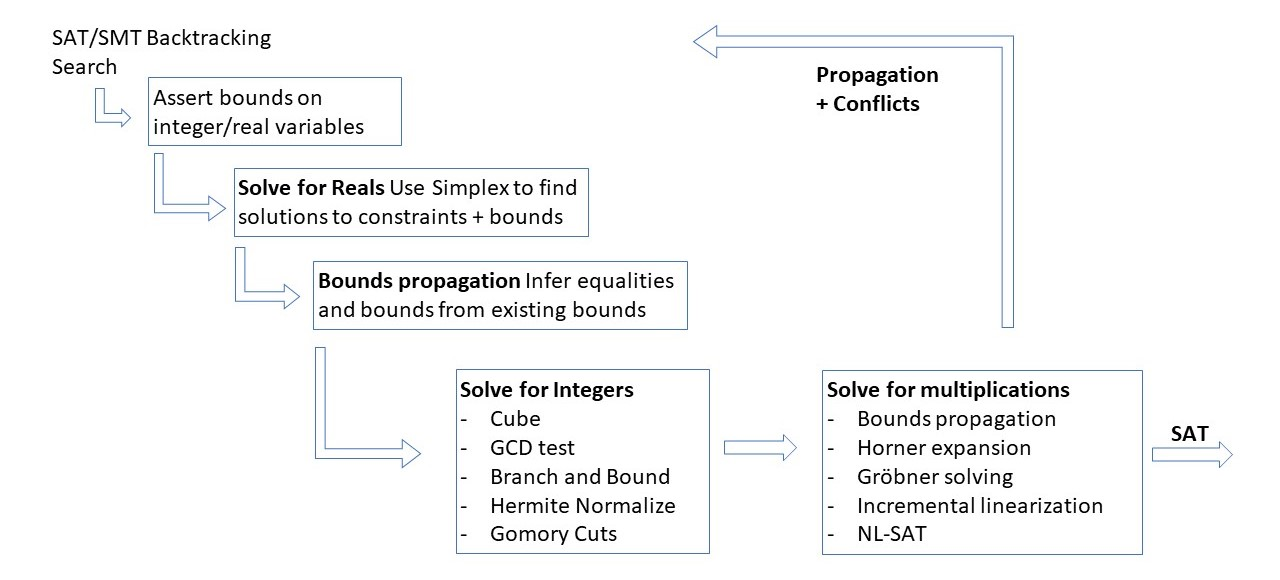
\includegraphics[width=0.99\textwidth]{figures/Arithmetic.jpg}
  \caption{Overview of Z3's Arithmetic Theory Solver }
  \label{fig:organization}
\end{figure}

The rest of the paper elaborates on the components of the solver. For completeness, we
go through all relevant pieces. We highlight parts that to our knowledge are novel.

%In the following we will ``unpeal'' the onion comprising of the ingredients in
%each of the three phases and also how they are integrated.
%The overall behavior of the arithmetic solver is a combination of many parts;
%an advance in each part contributes to the overall advance of the solver.
%For benchmarks from applications we observe that there is no single component that
%is single-handedly responsible for ``cracking the code''.

\papercomment{
\begin{tikzpicture}[node distance=2cm]
    \node (start) [startstop] {SAT/SMT Backtracking Search};
    \node (pro1) [process, below of=start, right of=start] {\begin{tabular}{l}Assert bounds on \\ integer/real variables\end{tabular}};
    \node (pro2) [process, below of=pro1, right of=pro1, yshift=-0.5cm] {\begin{tabular}{l}Solve for Reals Use Simplex to find \\ solutions to constraints + bounds\end{tabular}};
    \node (pro3) [process, below of=pro2, right of=pro2, yshift=-0.5cm] {\begin{tabular}{l} Bounds propagation Infer equalities and \\ bounds from existing bounds\end{tabular}};
    \node (pro4) [process, right of=pro3, right of=pro3, xshift=3cm] {Propagation + Conflicts};
    \node (pro5) [process, below of=pro4, yshift=-0.5cm] {\begin{tabular}{l}Solve for Integers\\
        Cube, \\
        GCD test, \\
        Branch and Bound, \\
        Hermite Normalize, \\
        Gomory Cuts
    \end{tabular}};
    \node (pro7) [process, right of=pro5, xshift=3cm] {Propagation + Conflicts};
    \node (pro8) [process, below of=pro5, yshift=-0.5cm] {\begin{tabular}{l}Solve for multiplications\\
        Bounds propagation, \\
        Horner expansion, \\
        Gr{\"o}bner solving, \\
        Incremental linearization, \\
        NL-SAT
    \end{tabular}};
    \node (end) [startstop, below of=pro8] {SAT};
    \draw [arrow] (start) -- (pro1);
    \draw [arrow] (pro1) -- (pro2);
    \draw [arrow] (pro2) -- (pro3);
    \draw [arrow] (pro3) -- (pro4);
    \draw [arrow] (pro3) -- (pro5);
    \draw [arrow] (pro5) -- (pro7);
    \draw [arrow] (pro7) -- (pro8);
    \draw [arrow] (pro8) -- (end);
\end{tikzpicture}
}


\papercomment{
  \subsection{Notes}

\begin{itemize}
  \item For a set of equations in form $x \pm y$ find fixed variables based on the variable values. Consider a graph formed by edges $(x,y)$, break it into connected components, and use pivoting to transform each component into a star.

\end{itemize}
}
